% compile with XeLaTeX
\documentclass[dvipsnames,mathserif]{beamer}
\setbeamertemplate{footline}[frame number]
\setbeamercolor{footline}{fg=black}
\setbeamerfont{footline}{series=\bfseries}
\usepackage{tikz}
\usepackage{adjustbox}
\usepackage{subcaption}
\usepackage{graphicx}
\usepackage{verbatim}
\usepackage{colortbl}
\usepackage{booktabs}% http://ctan.org/pkg/booktabs
\usepackage{subcaption}
\usepackage{fancyvrb}
\usepackage[utf8]{inputenc}

\usepackage{subcaption}
\usepackage{tikz}

\newcommand{\trianglesubfigures}[3]{%
  \begin{tikzpicture}
    \node[inner sep=0pt, outer sep=0pt] (a) at (0, 0) {\subcaptionbox{\footnotesize{Loss Curves}}{\includegraphics[width=0.45\textwidth]{#1}}};
    \node[inner sep=0pt, outer sep=0pt] (b) at (5, 0) {\subcaptionbox{\footnotesize{Accuracy Curves}}{\includegraphics[width=0.45\textwidth]{#2}}};
    \node[inner sep=0pt, outer sep=0pt] (c) at (2.5, 3.464) {\subcaptionbox{\footnotesize{AUC Curves}}{\includegraphics[width=0.45\textwidth]{#3}}};
  \end{tikzpicture}
}

%\usetheme{Frankfurt}%1
\usetheme{Darmstadt}%1

% for RTL liste
\makeatletter
\newcommand{\RTListe}{\raggedleft\rightskip\leftm}
\newcommand{\leftm}{\@totalleftmargin}
\makeatother

% RTL frame title
\setbeamertemplate{frametitle}
{\vspace*{-1mm}
  \nointerlineskip
  \begin{beamercolorbox}[sep=0.3cm,ht=2.2em,wd=\paperwidth]{frametitle}
    \vbox{}\vskip-2ex%
    \strut\hskip1ex\insertframetitle\strut
    \vskip-0.8ex%
  \end{beamercolorbox}
}
% align subsection in toc
\makeatletter
\setbeamertemplate{subsection in toc}
{\leavevmode\rightskip=5ex%
  \llap{\raise0.1ex\beamer@usesphere{subsection number projected}{bigsphere}\kern1ex}%
  \inserttocsubsection\par%
}
\makeatother

% RTL triangle for itemize
\setbeamertemplate{itemize item}{\tiny\raise1.25pt\hbox{\donotcoloroutermaths$\blacktriangleleft$}}

%\setbeamertemplate{itemize item}{\rule{4pt}{4pt}}

\defbeamertemplate{enumerate item}{square2}
{\LR{
    %
    \hbox{%
      \usebeamerfont*{item projected}%
      \usebeamercolor[bg]{item projected}%
      \vrule width2.25ex height1.85ex depth.4ex%
      \hskip-2.25ex%
      \hbox to2.25ex{%
        \hfil%
        {\color{fg}\insertenumlabel}%
      \hfil}%
    }%
}}

\setbeamertemplate{enumerate item}[square2]
\setbeamertemplate{navigation symbols}{}


\titlegraphic {
  \begin{tikzpicture}[overlay,remember picture, opacity=0.1,]
    \node[] at (0, 2.9){
        
\includegraphics[width=0.63\textwidth]{udglogo.png}
  };\end{tikzpicture}}
  \setbeamertemplate{caption}[numbered]
  \begin{document}

  \rightskip\rightmargin
  \title{A Platform for Classifying Melanoma}
  \author{ \Large \textbf{Wilber Eduardo Bermeo Quito} }
  \institute{\large\textbf{Master in Data Science}\\
    ---------\\
    Higher Polytechnic School\\
    ---------\\
  University of Girona}
  \footnotesize{\date{\today }


    \begin{frame}
      \maketitle
    \end{frame}

    \begin{frame}{Summery}
      \footnotesize \tableofcontents

    \end{frame}

    \begin{frame}

      \[f^{\circ n} \equiv \underbrace{f \circ f \circ \ldots \circ f}_{n \text{ times}} \]

      \[succ \equiv \lambda n. \lambda f. \lambda x. f (n f x) \]

      \[zero \equiv \lambda f. \lambda x. x\]

      \[n \equiv \lambda f. \lambda x. f^{\circ n} x\]

    \end{frame}

    \section{Introduction}


    \begin{frame}
      \frametitle{Introduction}

      \[(\lambda f. \lambda x. f^{\circ 1} x)\ succ\ zero\]

    \end{frame}


    \begin{frame}
      \large Motivations
      \vspace{0.25cm}

      \footnotesize
      \begin{itemize}
        \item Enhance AI\footnote{Artificial Intelligence.} knowledge.
        \item Automation as way to democratize access to research and AI solutions.
        \item CAD\footnote{Computer-Aided Diagnosis.} system are promising path
          towards medical automation.
      \end{itemize}
    \end{frame}


    \begin{frame}
      \large Objectives
      \vspace{0.25cm}

      \footnotesize
      \begin{itemize}
        \item Gain expertise in deep learning theory and its real-world
          applications.
        \item Explore and study the optimal approach for utilizing the distribution
          of dermoscopy images from the dataset during the training process.
        \item Propose and train deep learning models using transfer learning on ISIC\footnote{Skin Imaging Collaboration.}
          Challenge melanoma images.
        \item Create an easy deployment CAD infrastructure running in Docker,
          with the trained models, a user-friendly web UI\footnote{User
          Interface.} and a HTTP\footnote{Hypertext Transfer Protocol.} API\footnote{Application Programming Interface.}.
      \end{itemize}


    \end{frame}

    \section{Domain}

    \begin{frame}
      \frametitle{Domain}

      \[(\lambda f. \lambda x. f^{\circ 2} x)\ succ\ zero\]
    \end{frame}

    \begin{frame}
      \begin{center}
        \Huge Problem
      \end{center}
    \end{frame}


    \begin{frame}
      \large Detection of Melanoma Skin Cancer
      \vspace{0.25cm}

      \footnotesize
      \begin{itemize}
        \item Melanoma exhibits a high mortality rate.
        \item Dermoscopy procedures are utilized for melanoma detection.
        \item Dermoscopy images are examined by professionals to study cutaneous lesions.
        \item Several studies have shown that melanoma task classification
          using CAD systems achieve comparable or superior results to
          dermatologists.
      \end{itemize}


    \end{frame}


    \begin{frame}
      \begin{center}
        \Huge Solution
      \end{center}
    \end{frame}


    \begin{frame}

      \large CAD Training and Deployment Pipeline
      \vspace{0.25cm}

      \begin{figure}[H]
        %\begin{adjustbox}{width=\textwidth, trim={0.2cm 0pt 1.5cm 0pt}, clip}
        \centering
        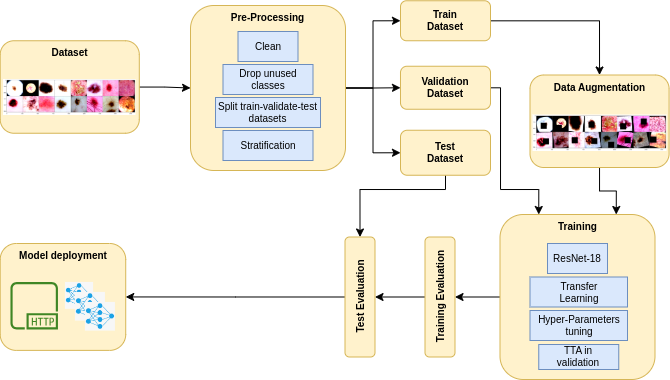
\includegraphics[width=0.7\textwidth]{images/Pipeline.drawio.png}
        %\end{adjustbox}
        \caption[CAD Infrastructure Pipeline]{\textit{CAD Infrastructure Pipeline.}}
        {\label{fig:cad-infrastructure-training-system}}
      \end{figure}

    \end{frame}

    \begin{frame}
      \large Micro-Service Architecture to Infer Images
      \vspace{0.25cm}

      \begin{figure}[H]
        \centering
        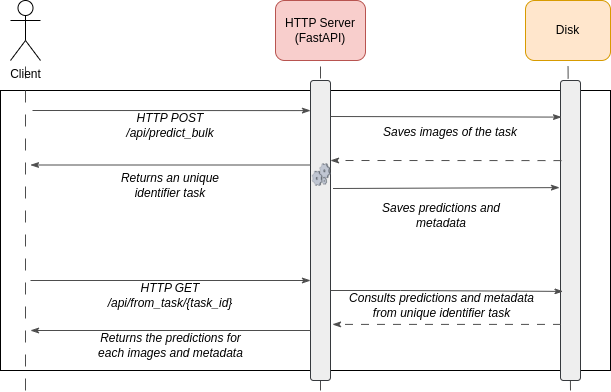
\includegraphics[width=0.65\textwidth]{images/BackgroundTask.drawio.png}
        \caption[Inferring Images Through the Background Task Mechanism]{\textit{Inferring Images Through the Background Task Mechanism.  }}
        {\label{fig:backgrond-task}}
      \end{figure}

    \end{frame}





    \section{Concerns}


    \begin{frame}
      \frametitle{Concerns}

      \[(\lambda f. \lambda x. f^{\circ 3} x)\ succ\ zero\]
    \end{frame}

    \begin{frame}
      \large Ethical Concern
      \vspace{0.25cm}

      \footnotesize
      \begin{itemize}
        \item The solution employs "black box" models, lacking explain-ability.
        \item The thesis presents a CAD tool designed to aid human decision-making
          rather than being an autonomous decision-making system.
      \end{itemize}
    \end{frame}

    \begin{frame}

      \large Regulatory Framework
      \vspace{0.25cm}

      \footnotesize

      \begin{itemize}
        \item When dealing with medical images, obtaining signed consent is
          necessary for data publication.
        \item Recent research collaborations prioritize data sharing through
          de-identification methods to tackle these challenges.
        \item The thesis made use of the ISIC Archive database, which serves as
          a publicly accessible resource.
      \end{itemize}


    \end{frame}



    \section{Data}

    \begin{frame}
      \frametitle{Data}

      \[(\lambda f. \lambda x. f^{\circ 4} x)\ succ\ zero\]
    \end{frame}

    \begin{frame}

      \large Origin Data
      \vspace{0.25cm}

      \footnotesize

      \begin{itemize}
        \item The data originates from the ISIC Archive.
        \item It includes images from the years 2019 and 2020.
        \item The images are available in three different resolutions: 512x512,
          768x768, and 1024x1024 pixels.
        \item The dataset contains more than eight distinct classes.
      \end{itemize}

    \end{frame}


    \begin{frame}

      \large Used Data
      \vspace{0.25cm}

      \footnotesize

      \begin{itemize}
        \item Resolution selected: 512x512 pixels.
        \item The used dataset comprises 31,265 distinct image samples.
        \item Eight classes were selected to work with.
        \item Imbalanced dataset.
      \end{itemize}

    \end{frame}

    \begin{frame}

      \large Classes Distribution in the Dataset
      \vspace{0.25cm}

      \begin{figure}[H]
        \centering
        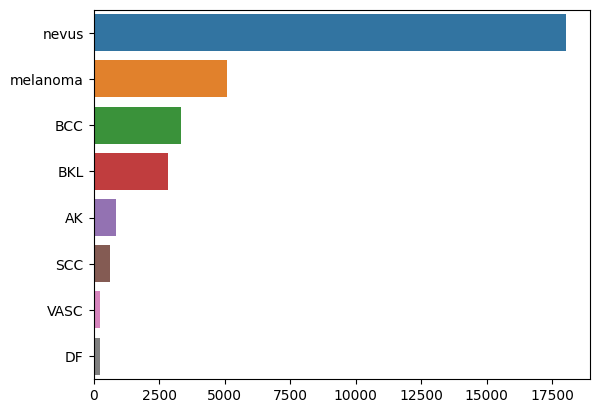
\includegraphics[width=0.7\textwidth]{images/hole-dataset-diagnosis.png}
        \caption[Data Distribution]{\textit{Data Distribution. }}
        {\label{fig:hole-dataset-distribution}}
      \end{figure}

    \end{frame}

    \begin{frame}

      \large  Train, Validation and Test Sets
      \vspace{0.25cm}

      \footnotesize

      \begin{itemize}
        \item The dataset was stratified to ensure an equal distribution of classes in each subset.
        \item The training set was created using 80\% of the dataset, the validation set using 10\%, and the test set using the remaining 10\%.
      \end{itemize}


      \begin{figure}[H]
        \centering
        \begin{adjustbox}{width=0.5\textwidth, trim={0cm 0.5cm 0cm 0.5cm}, clip}
          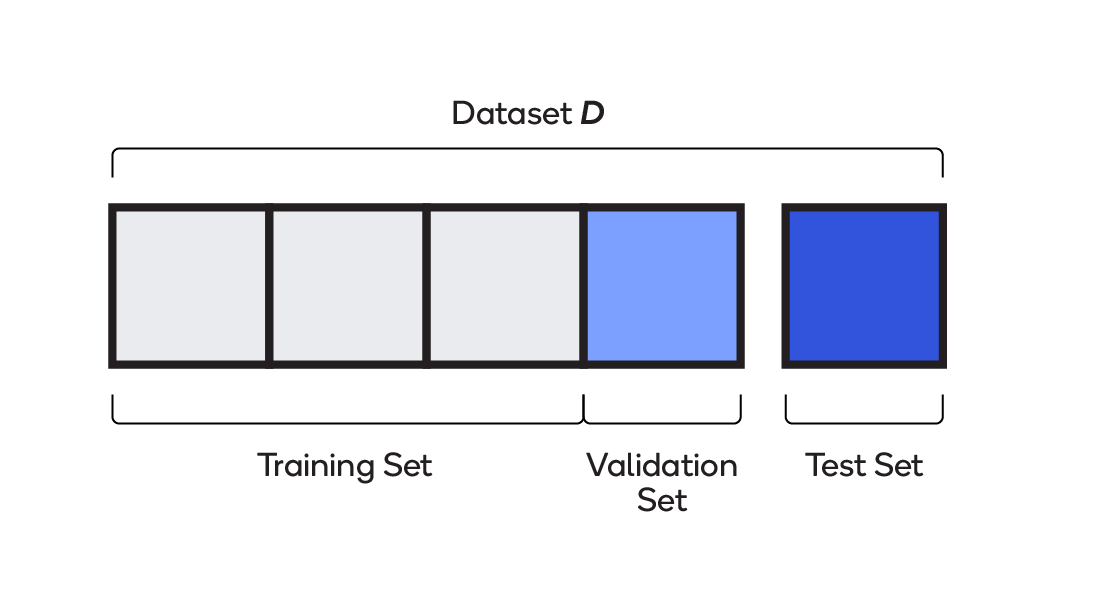
\includegraphics[width=\textwidth]{images/train-test-validation-sets.png}
        \end{adjustbox}
        \caption[Holdout Set Scheme]{\textit{Holdout Set Scheme. Illustration by Qualcomm}}
        {\label{fig:holdout-test-scheme}}
      \end{figure}

    \end{frame}

    \begin{frame}

      \large Data Augmentation
      \vspace{0.25cm}

      \footnotesize

      The train dataset (Figure \ref{fig:sample-of-datasets}),

      \begin{figure}[H]
        \centering
        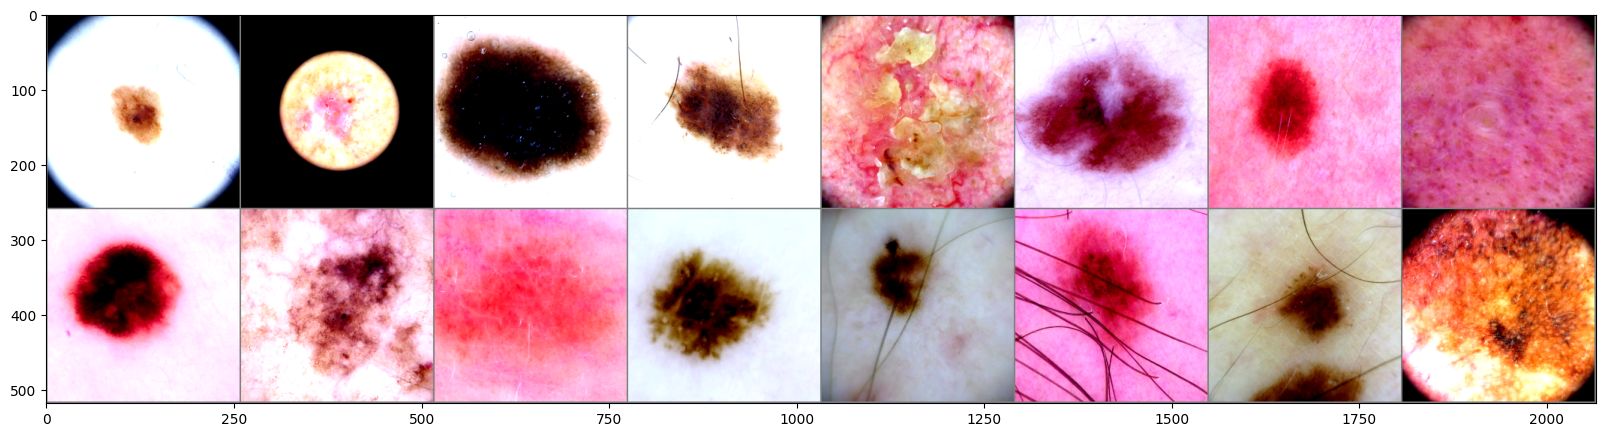
\includegraphics[width=0.6\textwidth]{images/random-sample-of-isic.png}
        \caption[Random Sample of Images]{\footnotesize{\textit{Random Sample of Images.}}}
        {\label{fig:sample-of-datasets}}
      \end{figure}

      Is mapped into an augmented train dataset (Figure \ref{fig:aug-sample-of-datasets}).

      \begin{figure}[H]
        \centering
        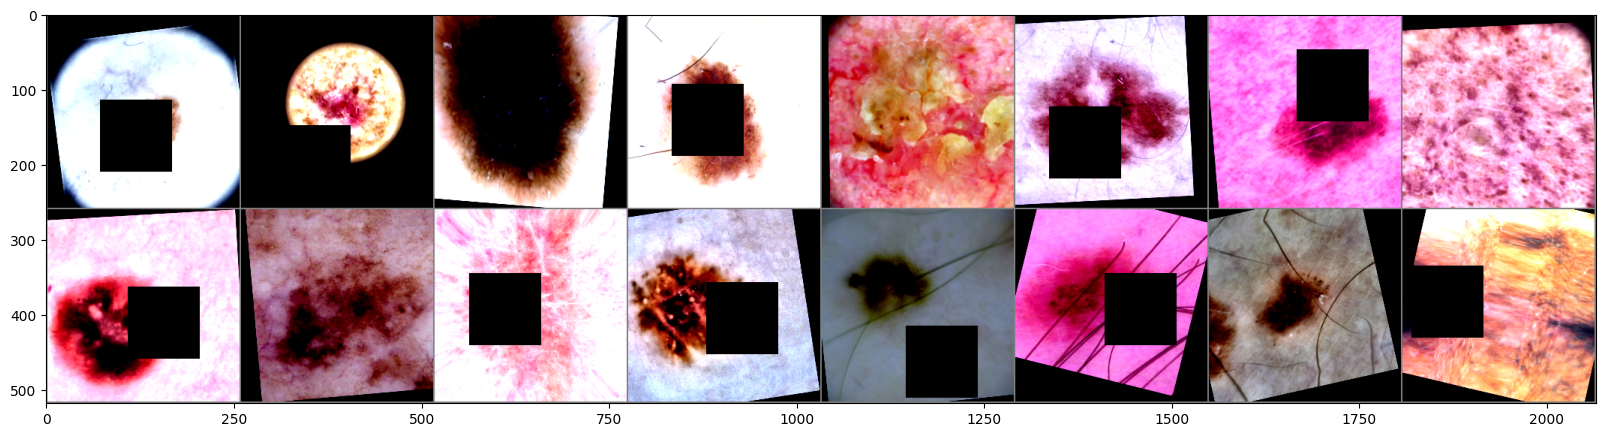
\includegraphics[width=0.6\textwidth]{images/random-sample-of-isic-augmented.png}
        \caption[Augmented Random Sample of Images]{\footnotesize{\textit{Augmented Random Sample of Images.}}}
        {\label{fig:aug-sample-of-datasets}}
      \end{figure}

    \end{frame}


    \section{Modeling}

    \begin{frame}
      \frametitle{Modeling}

      \[(\lambda f. \lambda x. f^{\circ 5} x)\ succ\ zero\]
    \end{frame}

    \begin{frame}

      \large General Modeling Information
      \vspace{0.25cm}

      \footnotesize

      \begin{itemize}
        \item Eight trained models with different ML\footnote{Machine Learning.} thecniques.
        \item Used the ResNet18 pre-trained weights.
        \item SGD\footnote{Stochastic Gradient Descent} as optimizer.
        \item Cross-entropy as loss function.
        \item Model training performance were evaluated with AUC\footnote{Area Under the Curve.} metric.
      \end{itemize}

    \end{frame}

    \begin{frame}


      \begin{table}

        \centering
        \begin{adjustbox}{width=\textwidth}
          \begin{tabular}{lcccccccc}
            \toprule
      & \textbf{M0} & \textbf{M1} & \textbf{M2} & \textbf{M3} & \textbf{M4} & \textbf{M5} & \textbf{M6} & \textbf{M7} \\
      \midrule
            Model Architecture & R18M & R18M & R18M & R18M & R18DM & R18DM & R18DM & R18DM \\
            Epochs & 20 & 20 & 20 & 20 & 40 & 40 & 40 & 40 \\
            Batch Size & 400 & 400 & 400 & 400 & 1024 & 1024 & 1024 & 1024 \\
            Scheduler & & SLR & CALR & CAWR &  & SLR & CALR & CAWR  \\
            Data Augmentation & No & No & No & No  & Yes & Yes & Yes & Yes \\
            Dropout Regularization & No & No & No & No  & Yes & Yes & Yes & Yes \\
            GPU & TT4 & TT4 & TT4 & TT4 & NA100 & NA100 & NA100 & NA100 \\
            Training Time & 1h 45m & 1h 22m & 1h 43m & 1h 38m & 1d 7h 30m & 1d 7h 4m & 1d 7h 1m & 1d 12h 55m \\ \bottomrule
          \end{tabular}
        \end{adjustbox}
        \caption[Training Information For Each Model.]
        {\textit{\footnotesize{Training Information For Each Model. Empty spaces represent non-use of that feature.}}}
        {\label{table:trained-models-information}}
      \end{table}

    \end{frame}


    \begin{frame}

      \begin{table}
        \centering
        \begin{adjustbox}{width=0.8\textwidth}
          \begin{tabular}{lccccccccc}
            \toprule
      & \textbf{Train AUC} & \textbf{Val AUC} & \textbf{Train Recall} & \textbf{Val Recall} & \textbf{Train Acc} & \textbf{Val Acc} \\
      \midrule
            M0 & 0.952 & 0.903 & 0.756 & 0.676  & 0.835 & 0.778 \\
            M1 $\star$ & 0.947 & 0.900 & 0.695 & 0.633 & 0.829 & 0.779 \\
            M2 $\ast$ & 0.933 & 0.895 & 0.658 & 0.609  & 0.808 & 0.765  \\
            M3 $\bullet$ & 0.935 & 0.896  & 0.663 & 0.605  & 0.811 & 0.767  \\
            \midrule
            \cellcolor{gray!50}M4 & \cellcolor{gray!50}0.886 & \cellcolor{gray!50}0.877 &  \cellcolor{gray!50}0.478 & \cellcolor{gray!50}0.475 &  \cellcolor{gray!50}0.757 & \cellcolor{gray!50}0.750 \\
            \cellcolor{gray!50}M5 $\star$ & \cellcolor{gray!50}0.867 & \cellcolor{gray!50}0.861  & \cellcolor{gray!50}0.423 & \cellcolor{gray!50}0.403 &  \cellcolor{gray!50}0.728 & \cellcolor{gray!50}0.717\\
            \cellcolor{gray!50}M6 $\ast$ & \cellcolor{gray!50}0.874 & \cellcolor{gray!50}0.868 & \cellcolor{gray!50}0.451 & \cellcolor{gray!50}0.440 & \cellcolor{gray!50}0.738 & \cellcolor{gray!50}0.728 \\
            \cellcolor{gray!50}M7 $\bullet$ & \cellcolor{gray!50}0.877  & \cellcolor{gray!50}0.849 & \cellcolor{gray!50}0.470 & \cellcolor{gray!50}0.432 & \cellcolor{gray!50}0.742 & \cellcolor{gray!50}0.732  \\

            \midrule

            Mean &  94.175\% & 89.850\%   & 69.300\% & 63.075\%  & 82.075\% & 77.225\%  \\
            SD   & 0.921\% & 0.370\%  &  4.509\% & 3.260\%  & 1.327\% & 0.727\%  \\

            \midrule

            \cellcolor{gray!50}Mean & \cellcolor{gray!50}87.600\% & \cellcolor{gray!50}86.875\% & \cellcolor{gray!50}45.550\% & \cellcolor{gray!50}44.400\% &  \cellcolor{gray!50}74.125\% & \cellcolor{gray!50}73.175\%  \\
            \cellcolor{gray!50}SD & \cellcolor{gray!50}0.787\% & \cellcolor{gray!50}0.655\% & \cellcolor{gray!50}2.445\% & \cellcolor{gray!50}3.084\% & \cellcolor{gray!50}1.204\% & \cellcolor{gray!50}1.372\% \\

            \bottomrule
          \end{tabular}
        \end{adjustbox}
        \caption[Train \& Validaton Metrics]
        {\textit{Train \& Validaton Metrics.}}
        {\label{table:resume-metrics}}
      \end{table}
    \end{frame}




    \begin{frame}
      \large M3 vs. M7

      \begin{figure}
        \centering
        \trianglesubfigures{images/LossM3M7.png}{images/AccM3M7.png}{images/AUCM3M7.png}
        \caption{\textit{M3 vs. M7. Combined AUC, Loss and Accuracy Curves.}}
        \label{fig:combined}
      \end{figure}
    \end{frame}

    \section{Workflow}


    \begin{frame}
      \frametitle{Workflow Methodology}

      \[(\lambda f. \lambda x. f^{\circ 6} x)\ succ\ zero\]
    \end{frame}

    \begin{frame}
      \begin{figure}[H]
        \centering
        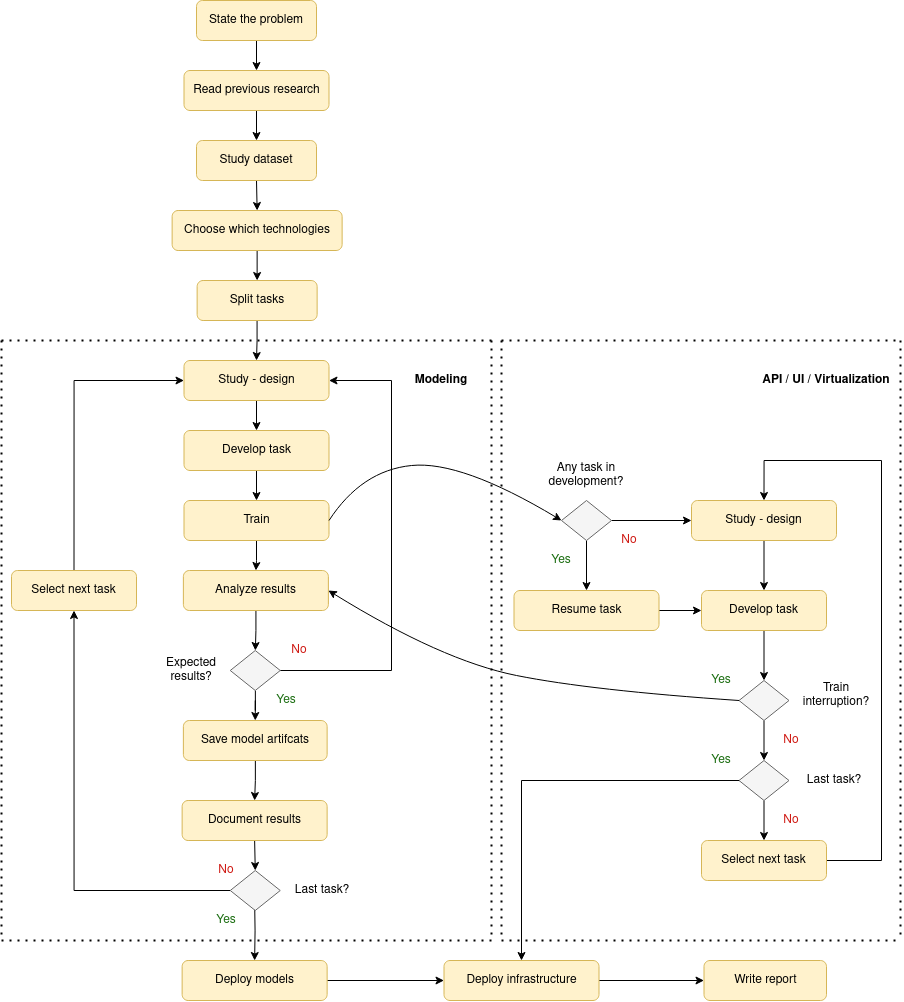
\includegraphics[width=0.6\textwidth]{images/EmplyedMethodology.png}
        \caption[Activity Diagram Describing the Methodology.]{\textit{Activity
        Diagram Describing the Workflow Methodology.}}
        {\label{fig:flux_development}}
      \end{figure}
    \end{frame}



    \section{Results}

    \begin{frame}
      \frametitle{Results}


      \[(\lambda f. \lambda x. f^{\circ 7} x)\ succ\ zero\]
    \end{frame}


    \begin{frame}
      \large Testing Models
      \vspace{0.25cm}
      \begin{figure}[H]
        \centering
        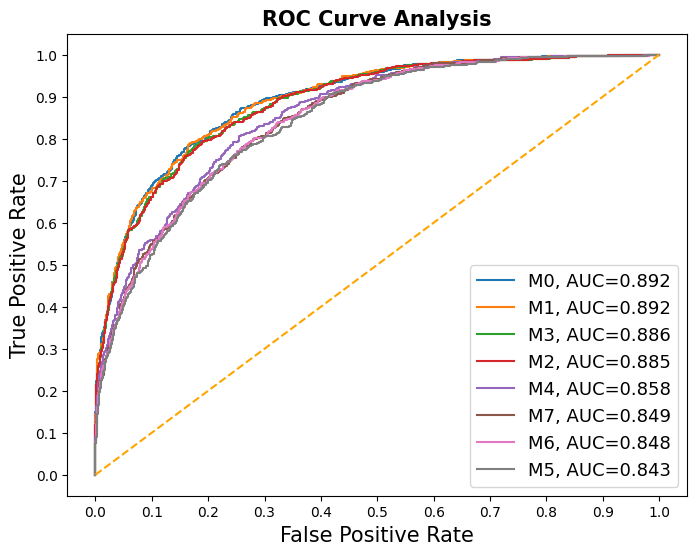
\includegraphics[width=0.65\textwidth]{images/rocaucanalysis-all.png}
        \caption[ROC-AUC Results in Test Dataset]{\textit{ROC-AUC Results in Test Dataset. }}
        {\label{fig:rocaucanalysis-all}}
      \end{figure}

    \end{frame}

    \begin{frame}[fragile]

      \large API Service
      \vspace{0.25cm}

      \footnotesize
      To access the documentation of the API, you can make a request in a web
      browser using the following URL\footnote{Uniform Resource Locator.}:

      \vspace{0.1cm}

      \begin{Verbatim}[fontsize=\tiny]
http://<api>/docs
      \end{Verbatim}

      The web browser will display the endpoints of the API.

      \begin{figure}[H]
        \centering
        \begin{adjustbox}{width=0.8\textwidth, trim={0cm 0cm 0.1cm 0cm}, clip}
          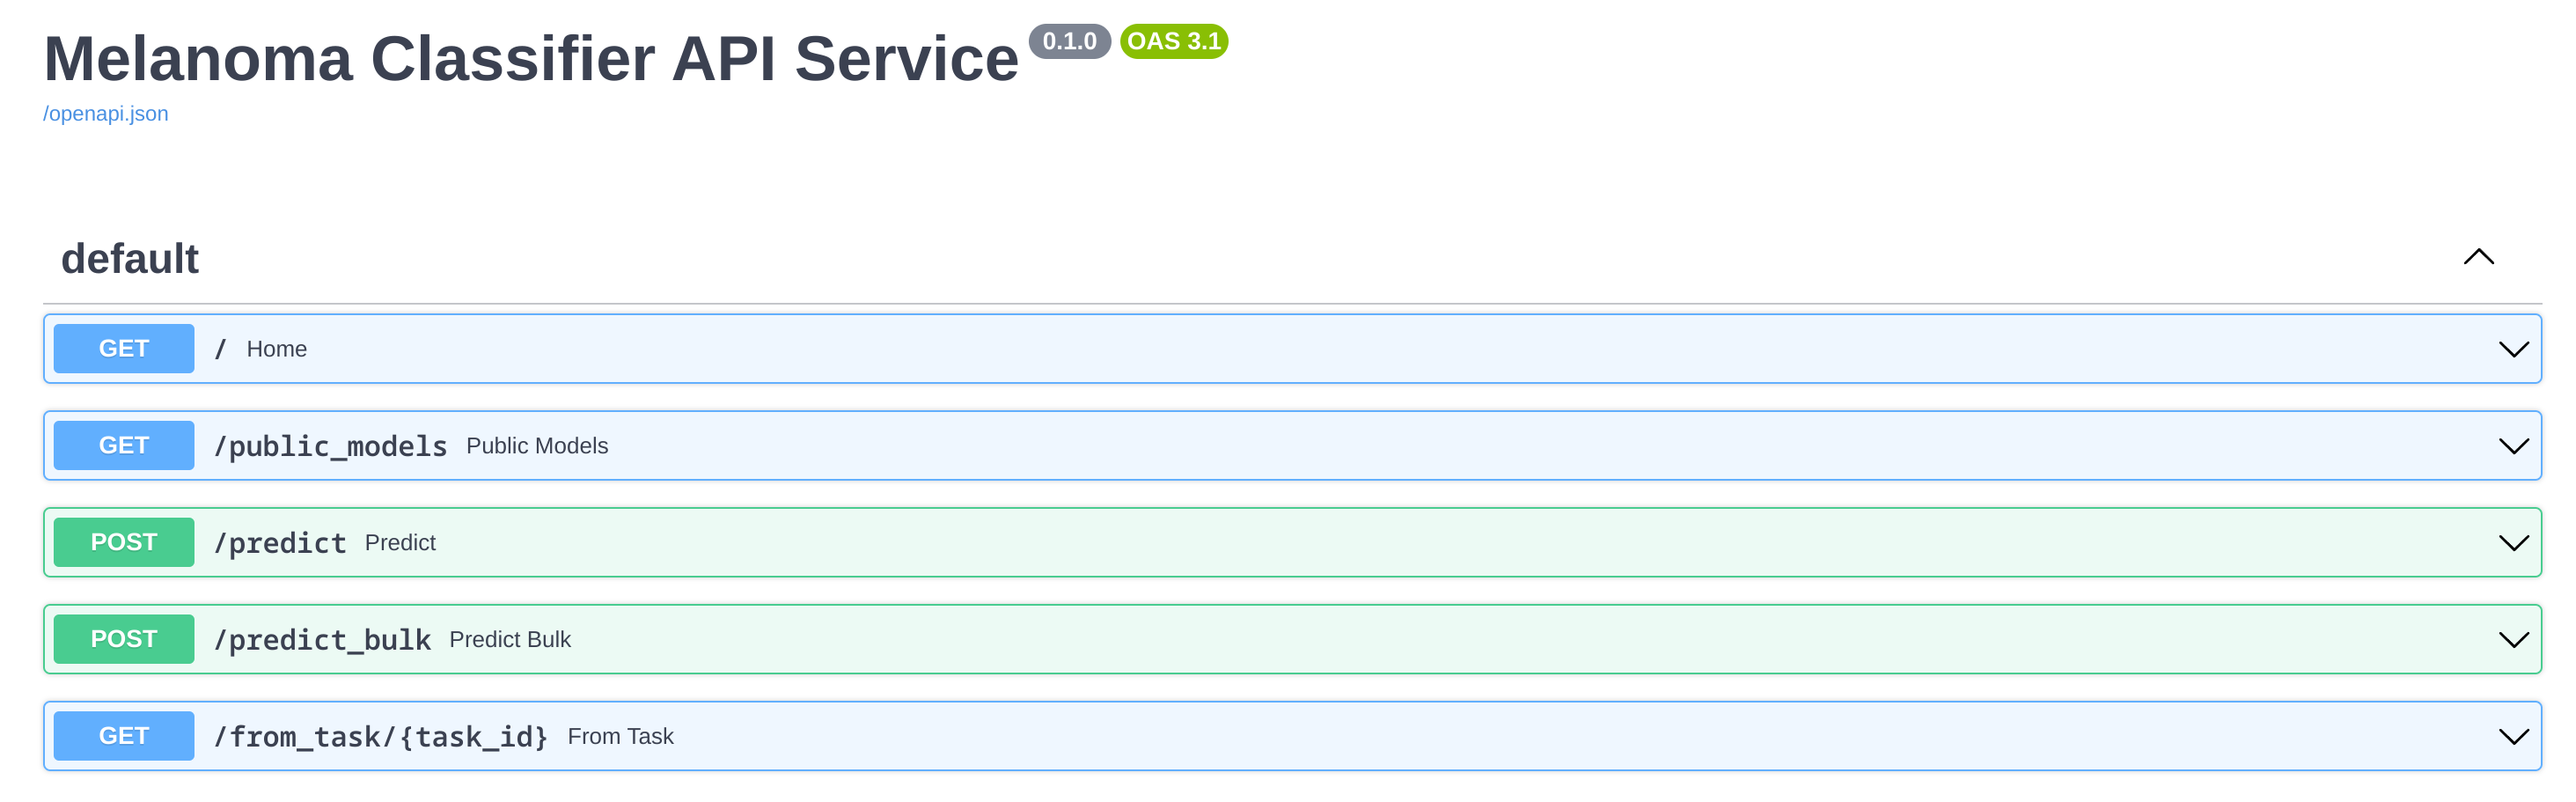
\includegraphics[width=\textwidth]{images/api-endpoints.png}
        \end{adjustbox}
        \caption[API Service End-Points]{\textit{API Service End-Points. }}
        {\label{fig:api-endpoints}}
      \end{figure}
    \end{frame}



    \begin{frame}[fragile]
      \large Exposed Models

      \vspace{0.25cm}
      \footnotesize
      You can consult the exposed models by requesting:

      \vspace{0.1cm}

      \begin{Verbatim}[fontsize=\tiny]
http://<api>/public_models
      \end{Verbatim}

      The response of the API's JSON\footnote{JavaScript Object Notation.}
      response should be something similar to this:

      \vspace{0.1cm}

      \begin{Verbatim}[fontsize=\tiny]
{
  "models": [
    "M0",
    "M1",
    "M2",
    "M3",
    "M4",
    "M5",
    "M6",
    "M7",
    "vicorobot.8c_b3_768_512_18ep_best_20_fold0",
    "vicorobot.8c_b3_768_512_18ep_best_fold0",
    "vicorobot.8c_b3_768_512_18ep_final_fold0"
  ]
}
      \end{Verbatim}

    \end{frame}


    \begin{frame}[fragile]
      \large Predict Images

      \vspace{0.25cm}
      \footnotesize
      You can consult the exposed models by requesting:

      \vspace{0.1cm}

      \begin{Verbatim}[fontsize=\tiny]
http://<api>/predict_bulk?model_id=<model_id>
      \end{Verbatim}
      The API will respond with a JSON object containing a unique task identifier and
      the total number of images sended to the API:

      \vspace{0.1cm}

      \begin{Verbatim}[fontsize=\tiny]
{
  "task_uuid": "77d5e834-60a1-49b6-a71a-b3472dc21ce5",
  "num_images": 2
}
      \end{Verbatim}

    \end{frame}

    \begin{frame}[fragile]
      \large Consult Prediction

      \vspace{0.25cm}
      \footnotesize
      You can consult a task prediction as follow:

      \vspace{0.1cm}

      \begin{Verbatim}[fontsize=\tiny]
http://<api>/from_task/<task_uuid>
      \end{Verbatim}

      A potential JSON response from the API regarding the task prediction:

      \vspace{0.1cm}

      \begin{Verbatim}[fontsize=\tiny]
[
  {
    "name": "ISIC_0052349.jpg",
    "probabilities": {
      "AK": 0.0007466986,
      "BCC": 0.0005002805,
      "BKL": 0.015733117,
      "DF": 0.00086343783,
      "SCC": 0.0007902466,
      "VASC": 0.0017217622,
      "melanoma": 0.017426228,
      "nevus": 0.9622182
    },
    . . .
  }
  . . .
]
      \end{Verbatim}

    \end{frame}


    \begin{frame}[fragile]
      \large UI Service
      \vspace{0.25cm}

      \footnotesize
      Accesing the UI service through a web browser using the following URL:

      \vspace{0.1cm}

      \begin{Verbatim}[fontsize=\tiny]
http://<ui>
      \end{Verbatim}

      As a result, a single-page web application with several interactive buttons will appear (Figure \ref{fig:ui-tools}).

      \vspace{0.2cm}
      The state of these button depends on the application state.


      \begin{figure}[H]
        \centering
        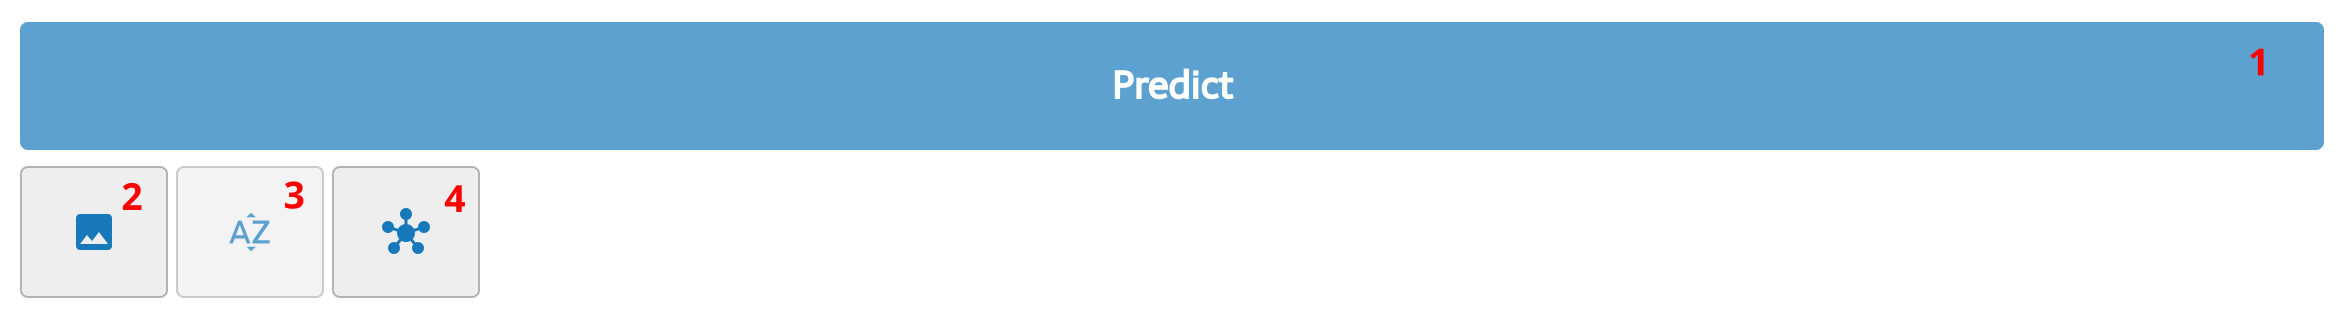
\includegraphics[width=\textwidth]{images/ui-tools.png}
        \caption[Main Interactive buttons of the UI Service]{\textit{Main Interactive buttons of the UI Service.}}
        {\label{fig:ui-tools}}
      \end{figure}

    \end{frame}


    \begin{frame}

      \begin{figure}[H]
        \centering
        \begin{adjustbox}{width=0.55\textwidth, trim={0cm 2.8cm 0cm 0cm}, clip}
          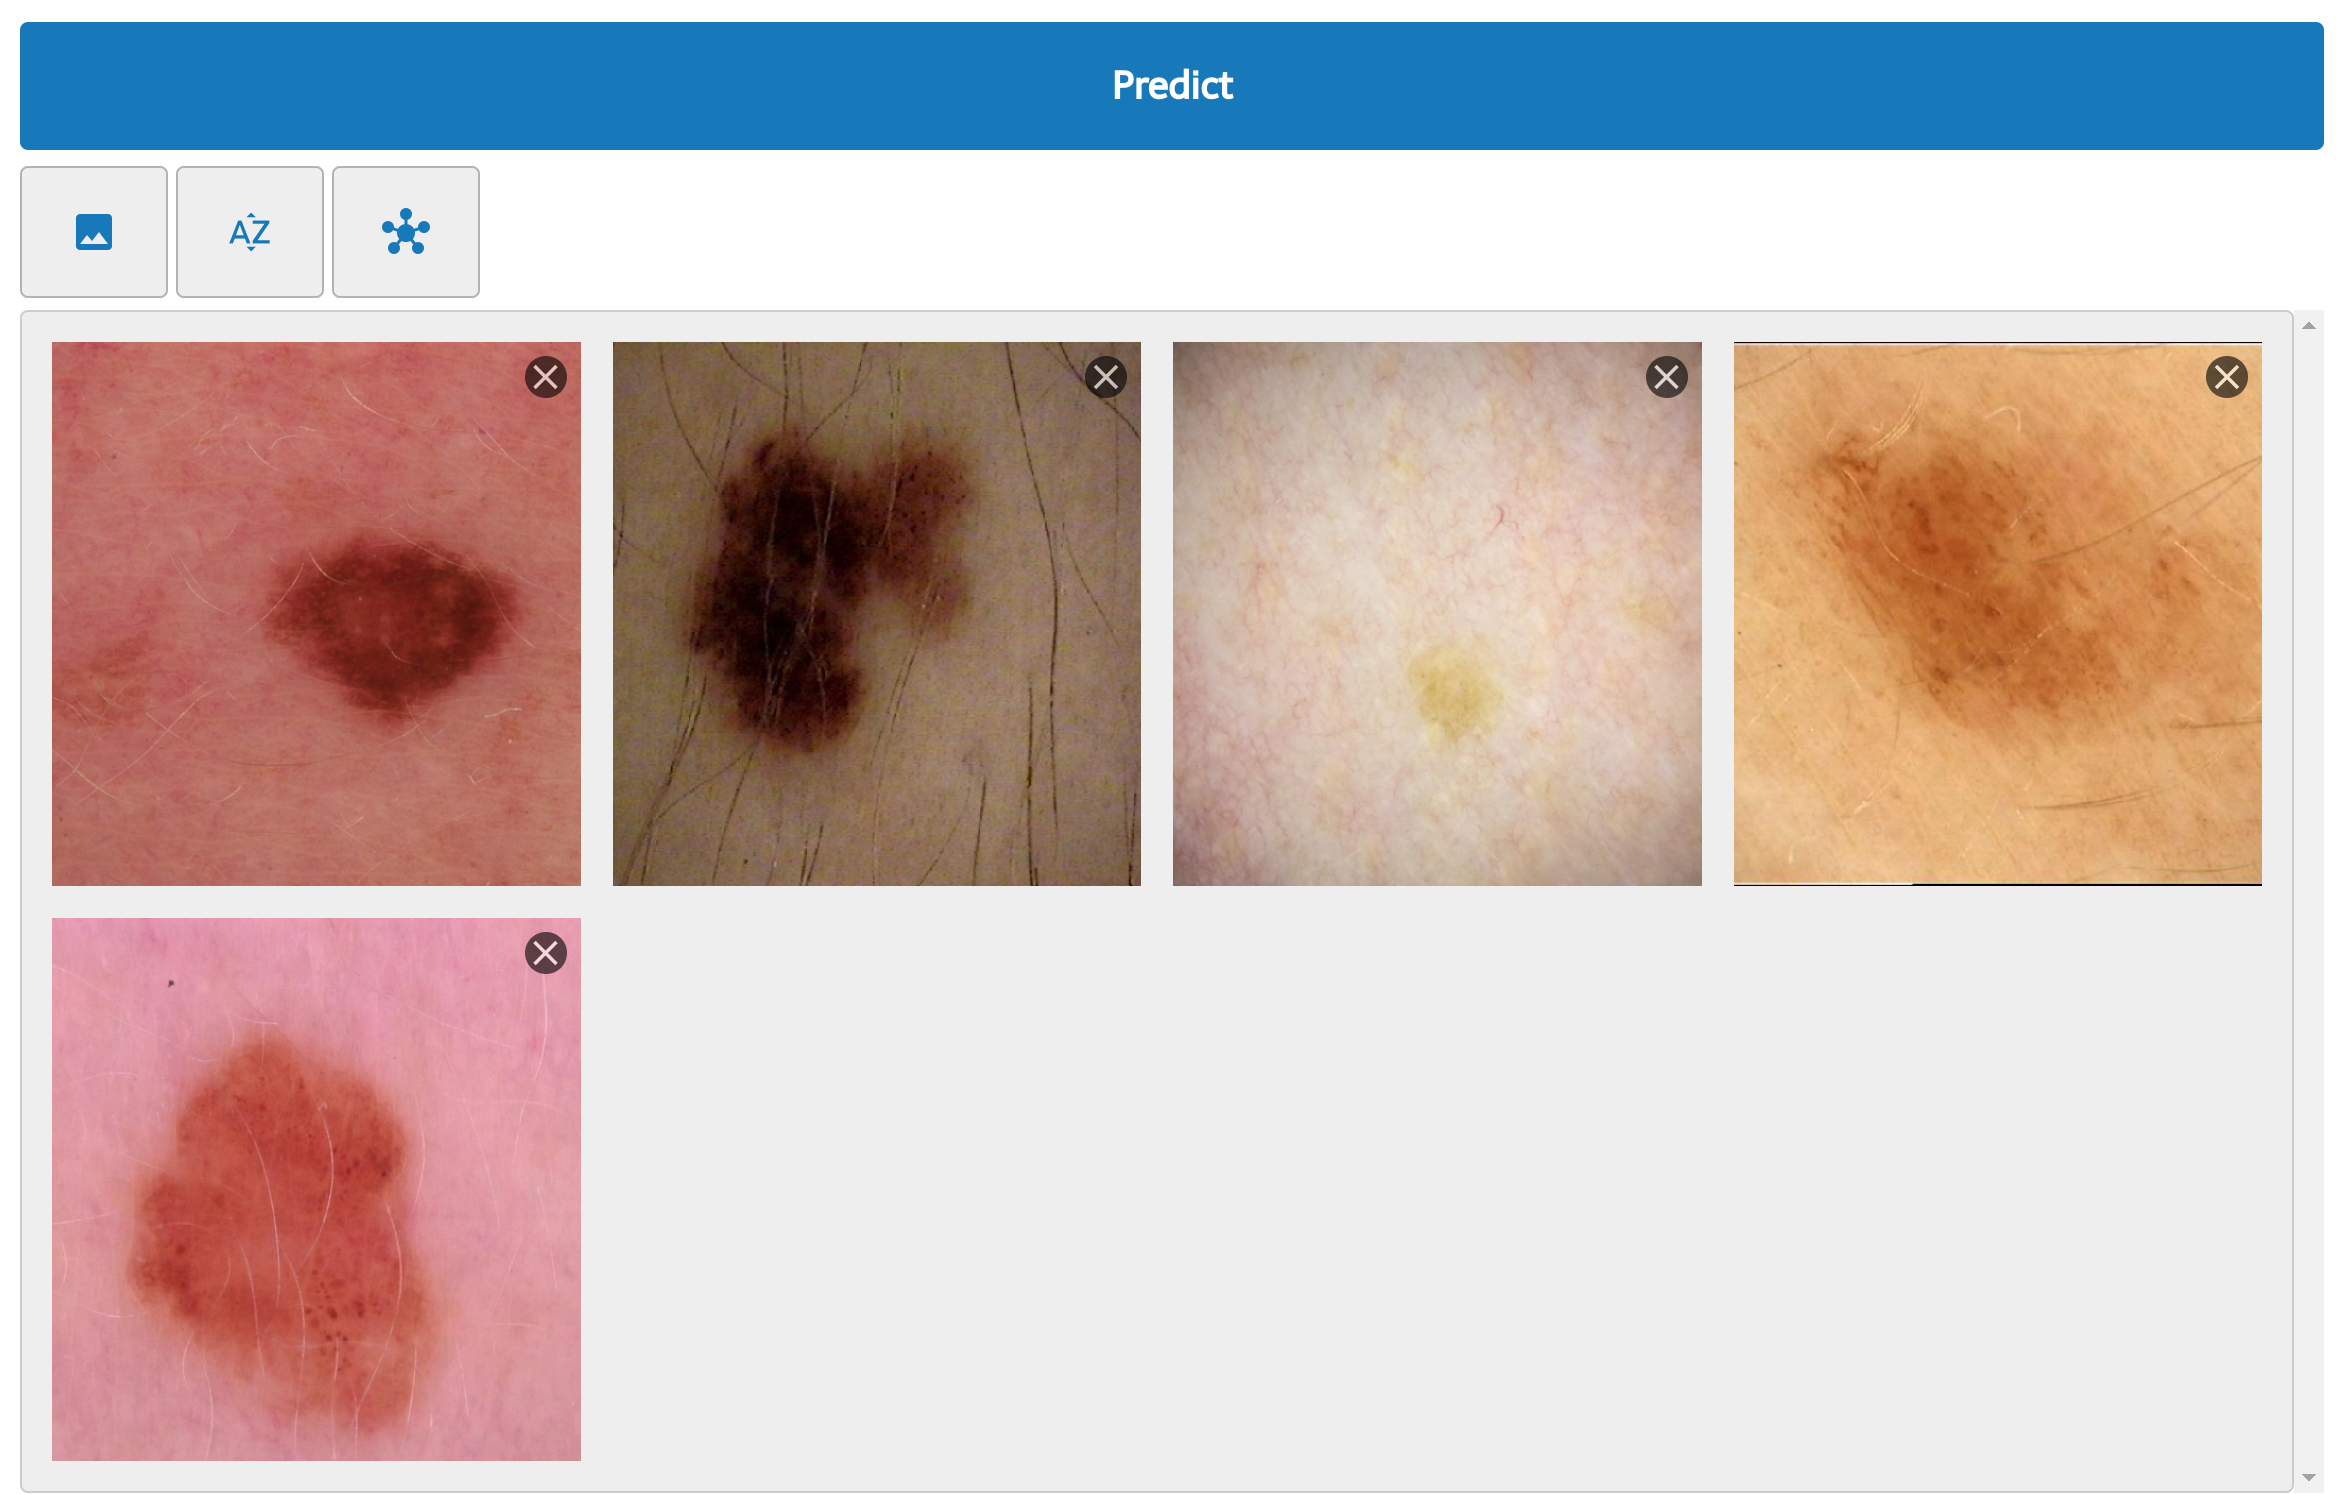
\includegraphics[width=\textwidth]{images/loaded-images.png}
        \end{adjustbox}
        \caption[Dermoscopy Images Loaded in the UI]{\footnotesize{\textit{Dermoscopy Images
        Loaded in the UI.}}}
        {\label{fig:loaded-images}}

        \begin{figure}[H]
          \centering
          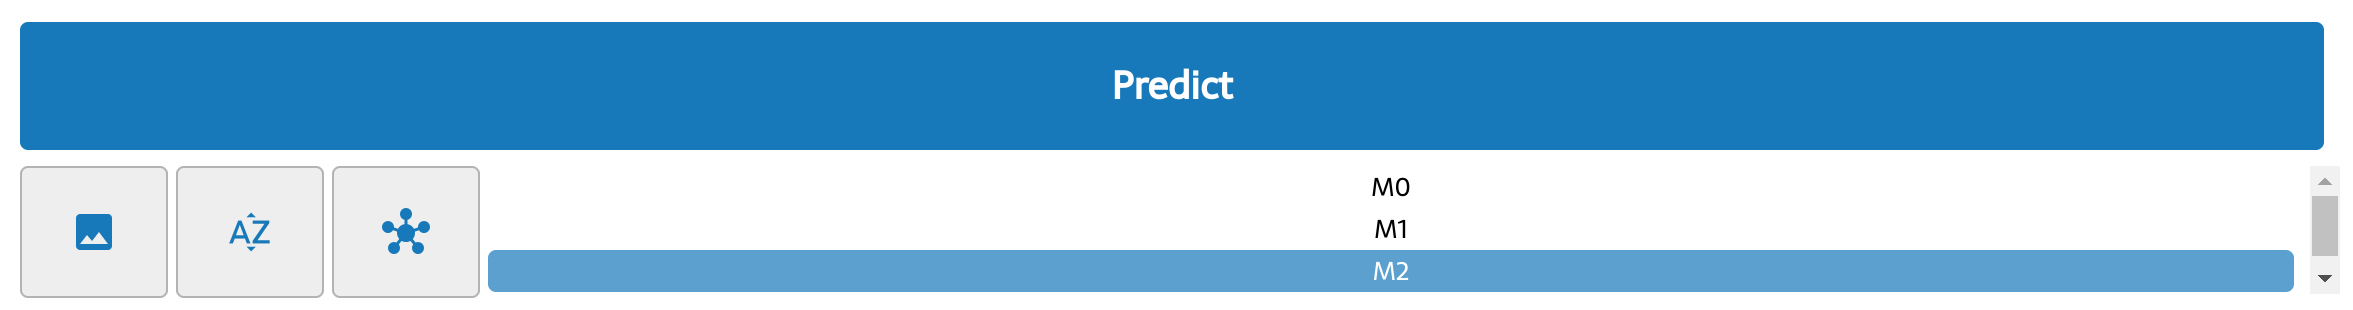
\includegraphics[width=0.55\textwidth]{images/selecting-model.png}
          \caption[Selecting Exposed Models by the API]{\footnotesize{\textit{Selecting
          Exposed Models by the API.}}}
          {\label{fig:selecting-model}}
        \end{figure}

        \begin{figure}[H]
          \centering
          \begin{adjustbox}{width=0.55\textwidth, trim={0cm 2.8cm 0cm 0cm}, clip}
            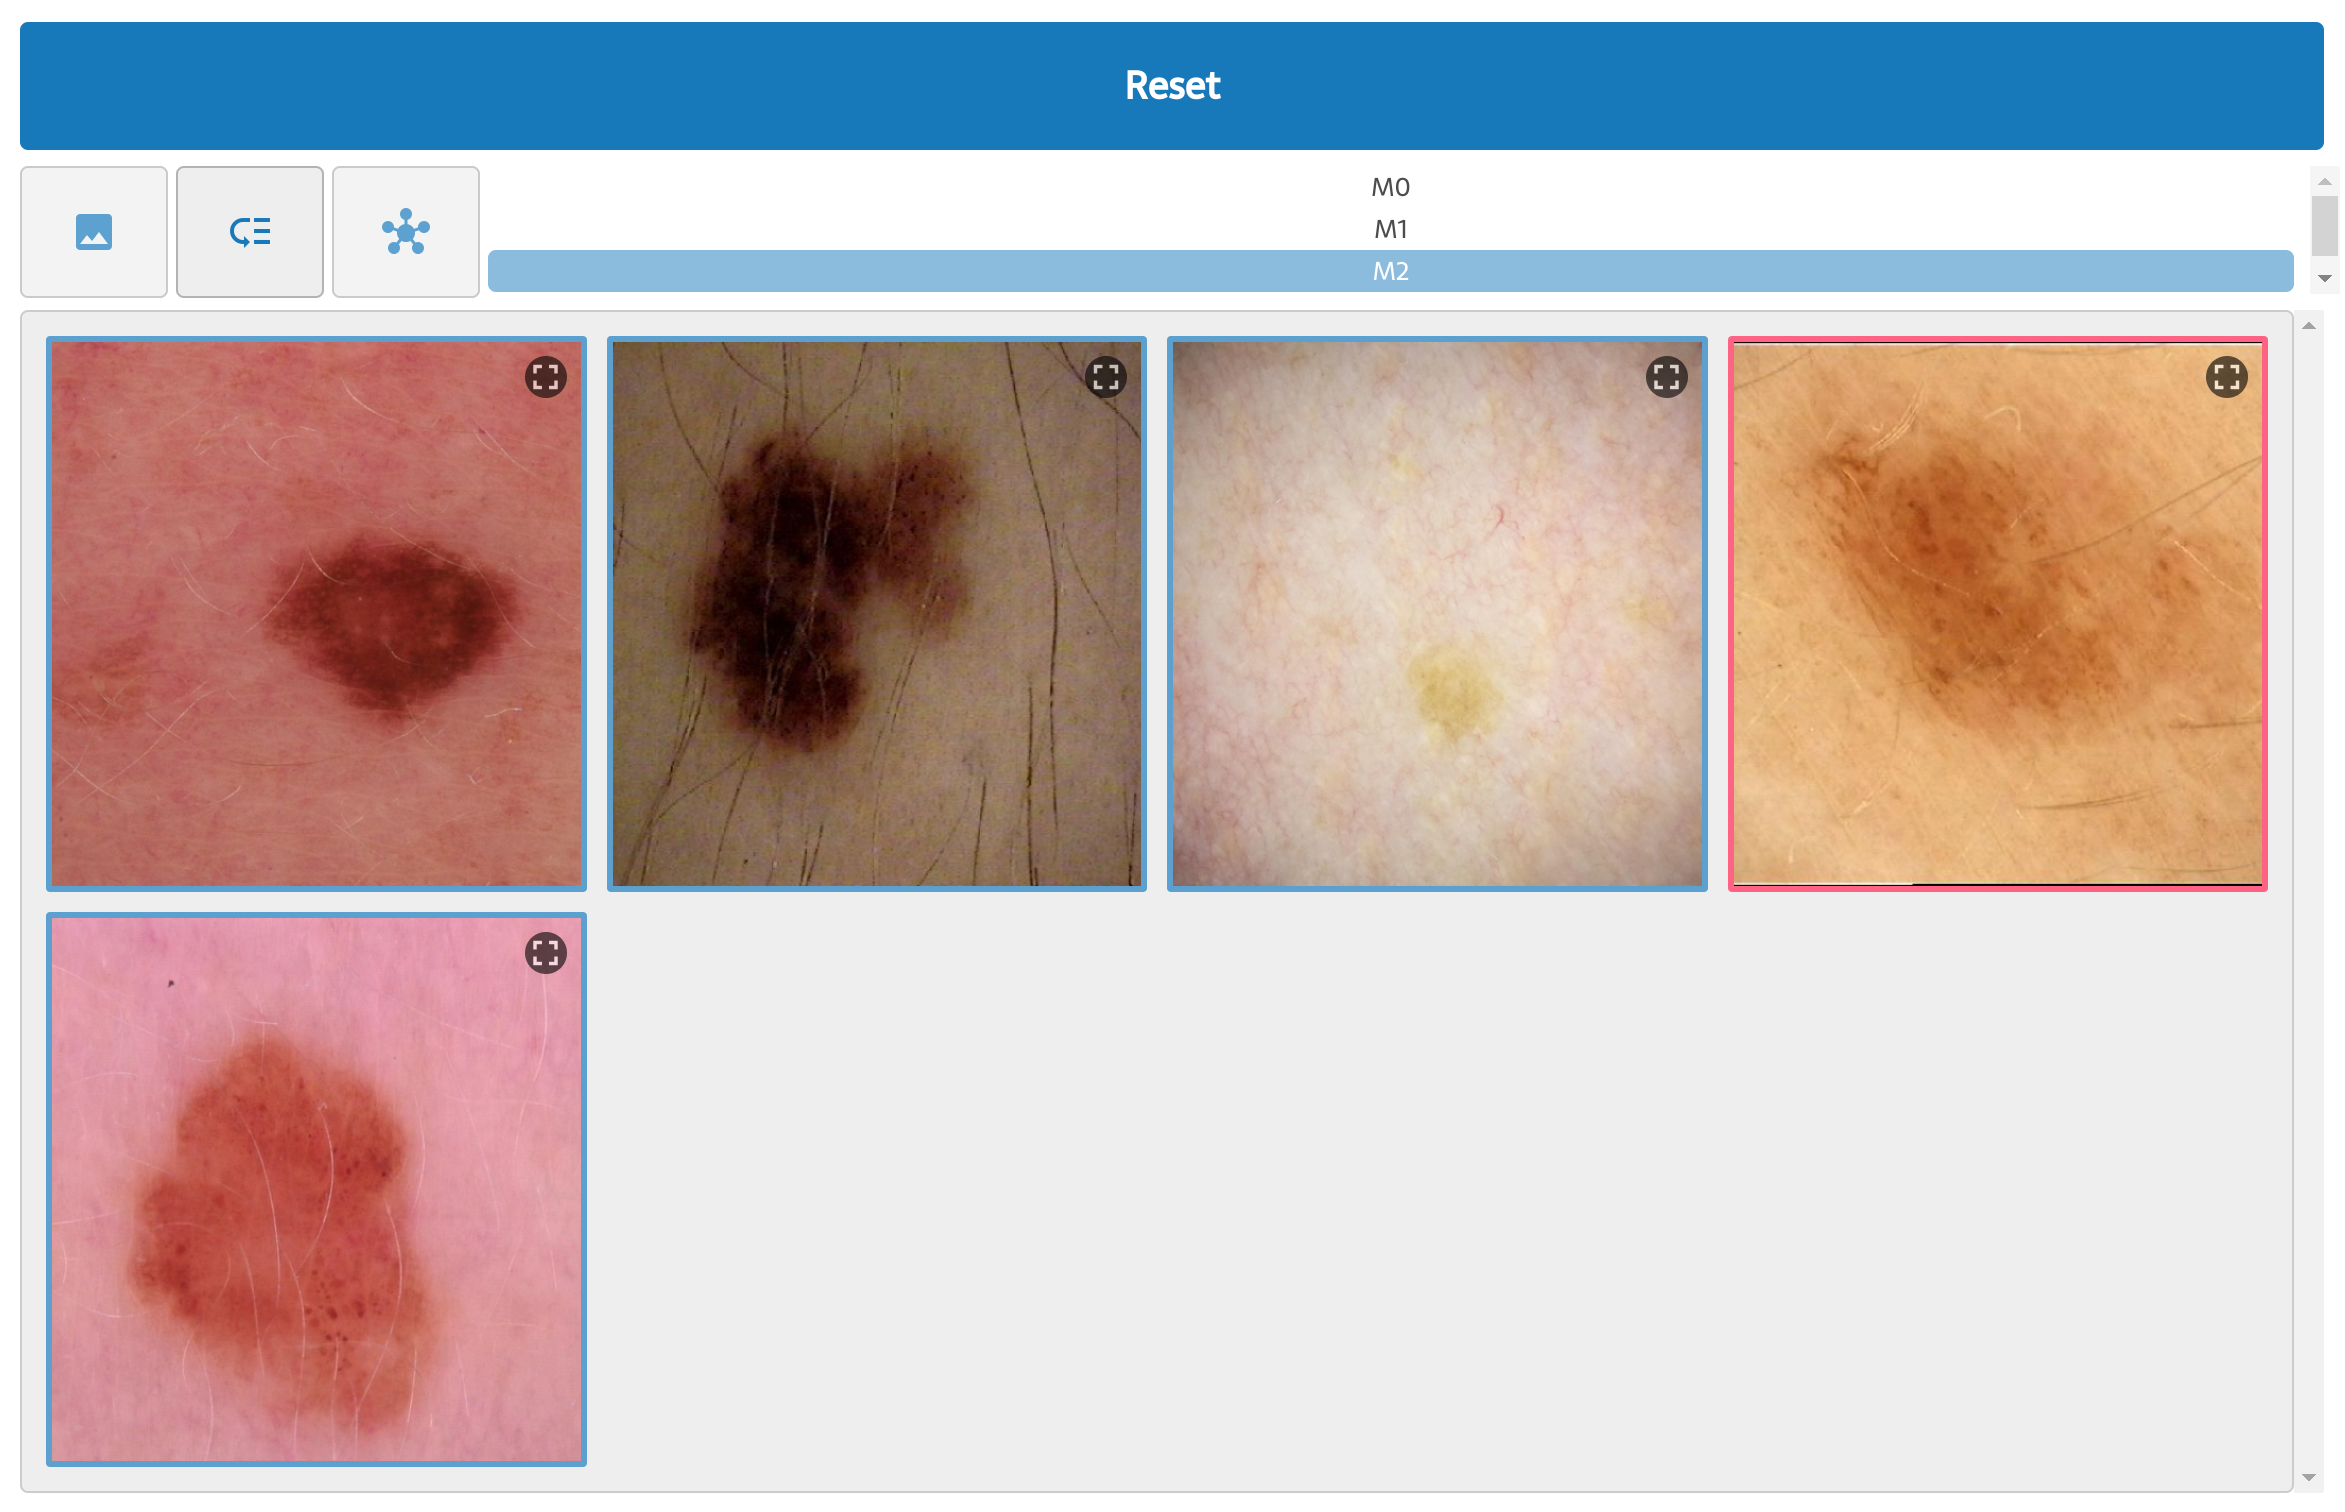
\includegraphics[width=\textwidth]{images/after-prediction.png}
          \end{adjustbox}
          \caption[UI State After Prediction Response]{\footnotesize{\textit{UI State After Prediction Response.}}}
          {\label{fig:after-prediction}}
        \end{figure}

      \end{figure}

    \end{frame}

    \begin{frame}

      \large Pop-up Extra Information
      \vspace{0.25cm}

      \begin{figure}[H]
        \centering
        \begin{adjustbox}{width=0.7\textwidth, trim={0.05cm 0cm 0.25cm 0cm}, clip}
          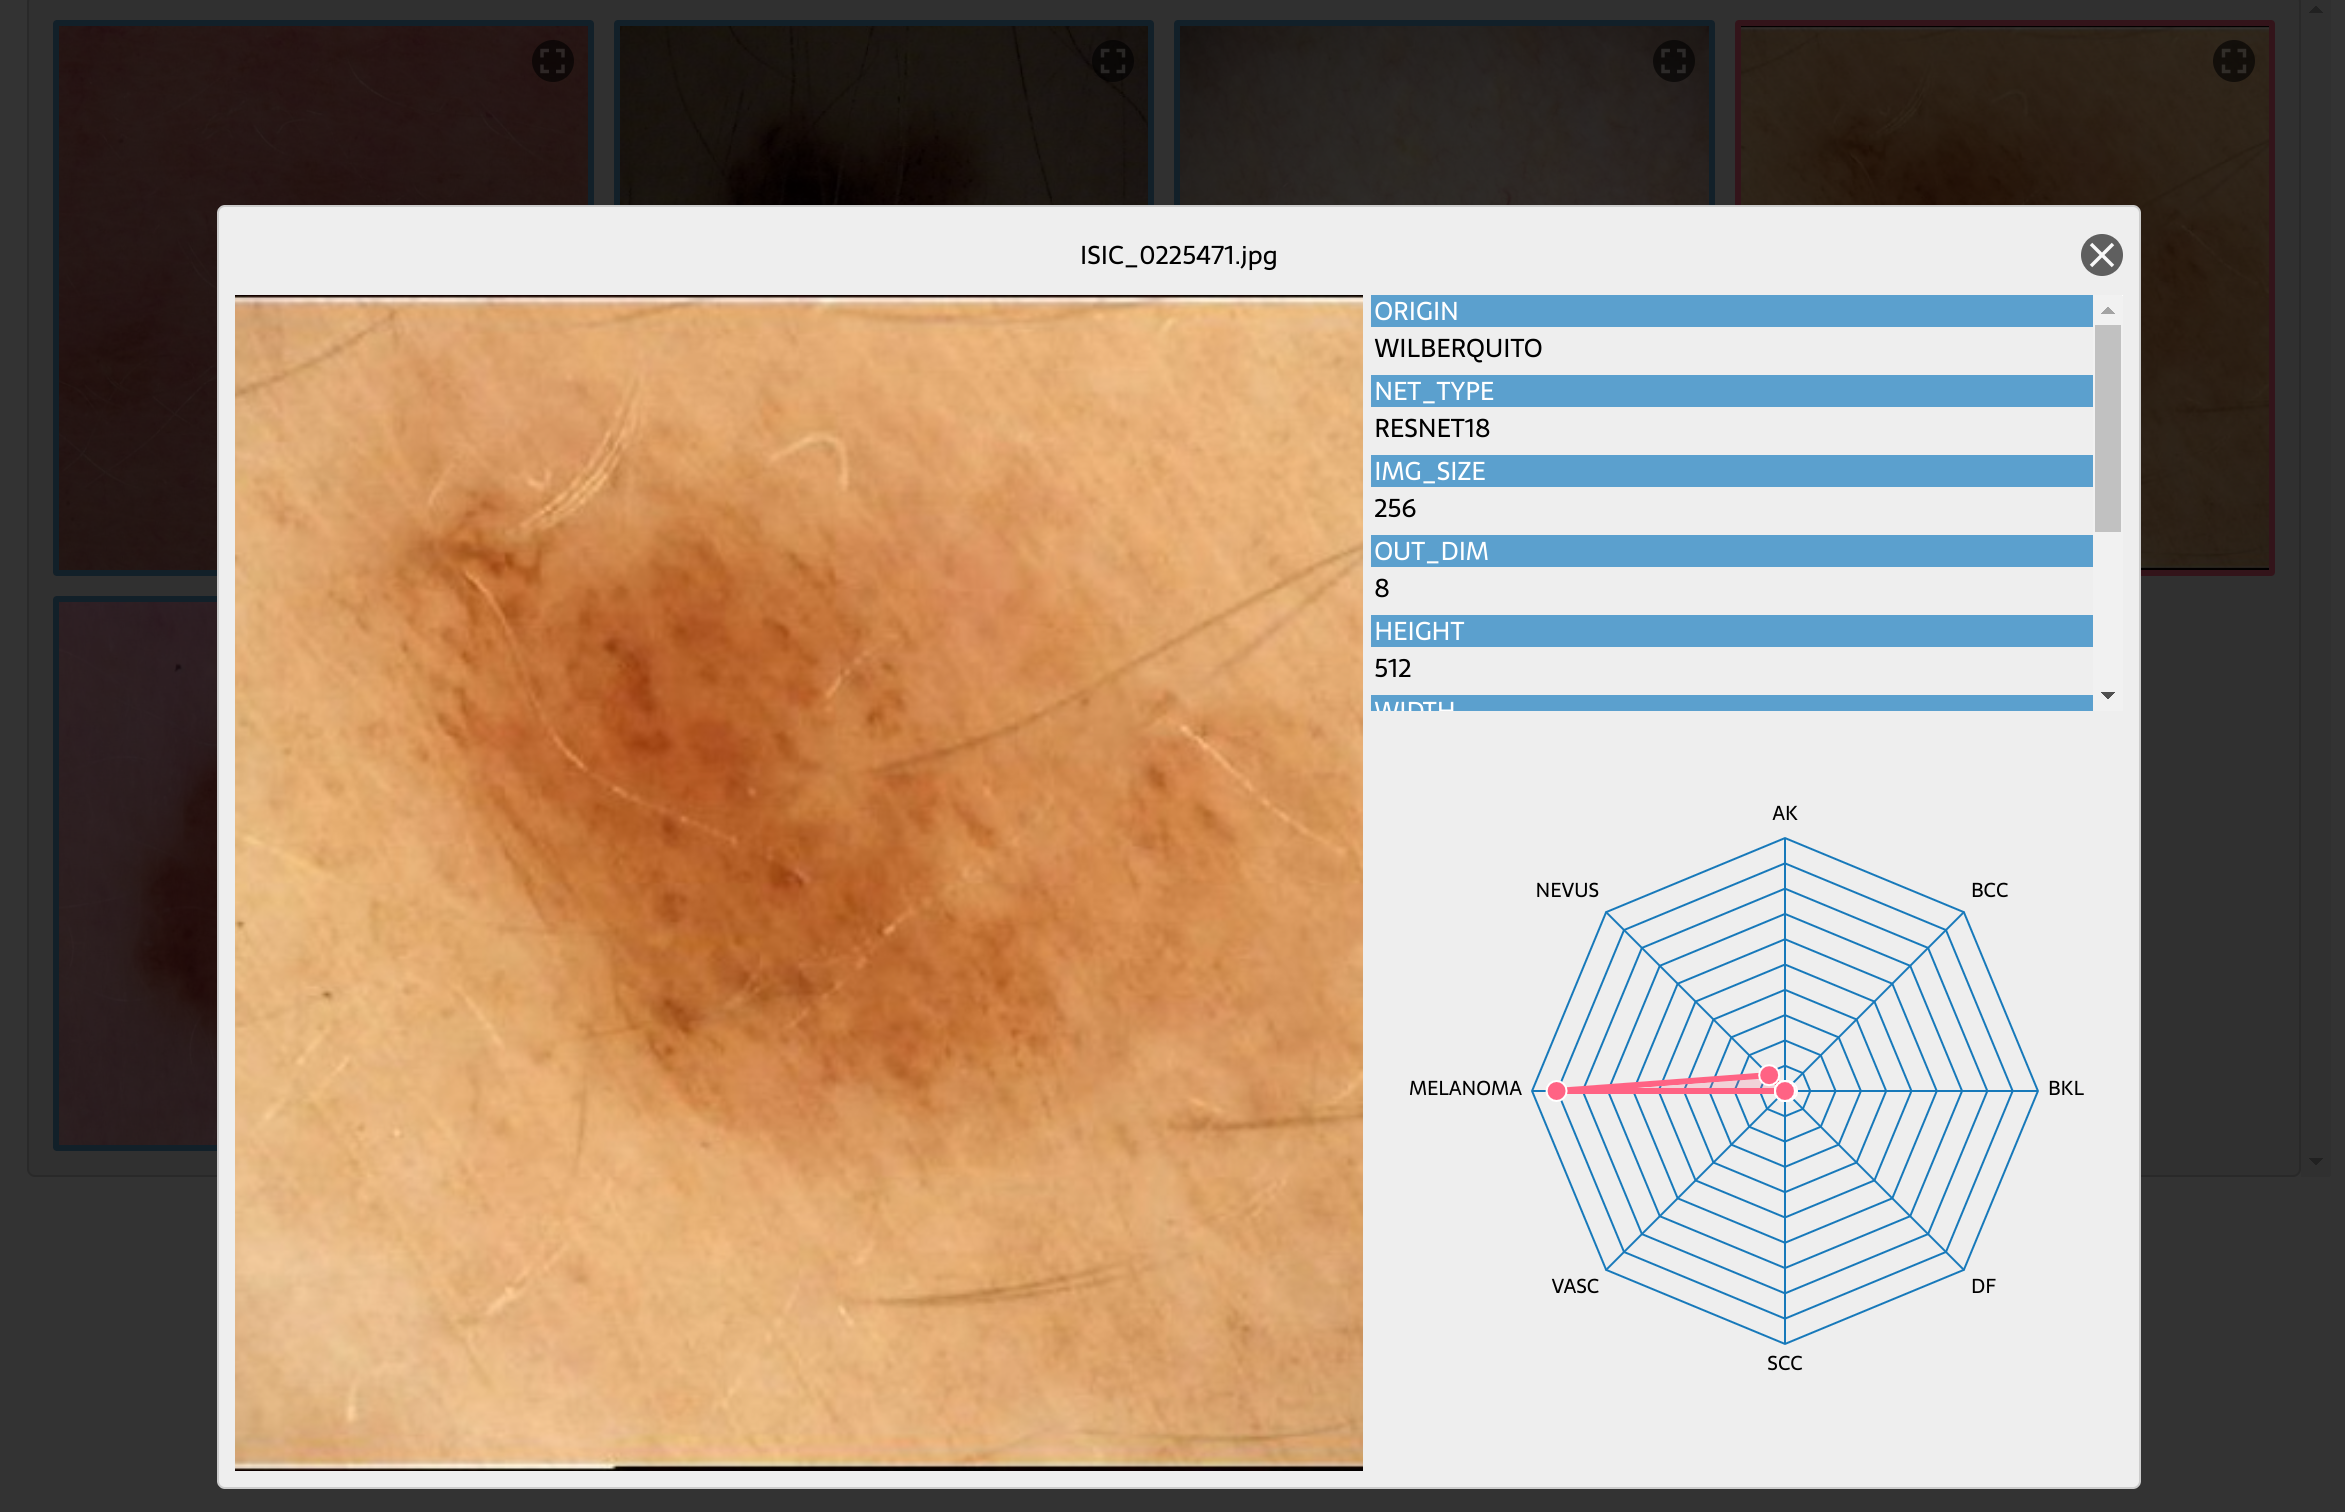
\includegraphics[]{images/extra-inf-popup.png}
        \end{adjustbox}
        \caption[Extra Prediction Information]{\textit{Extra Prediction Information.}}
        {\label{fig:extra-inf-popup}}
      \end{figure}

    \end{frame}


    \begin{frame}[fragile]


      \large Open Source CAD Infrastructure
      \vspace{0.25cm}

      \footnotesize

      The thesis assets (trained models weights and configurations) can be found in
      this public GitLab repository:

      \vspace{0.1cm}

      \begin{Verbatim}[fontsize=\tiny]
https://gitlab.com/wilberquito/open.thesis
      \end{Verbatim}

      The CAD infrastructure (install guide, install script, experiments and source code) can be found in
      this public GitHub repository:

      \vspace{0.1cm}

      \begin{Verbatim}[fontsize=\tiny]
https://github.com/wilberquito/melanoma.thesis
      \end{Verbatim}

      After following the instruction and installing the required tools, installing the CAD infrastructure should
      be as simple as running this command in a bash terminal.

      \vspace{0.1cm}

      \begin{Verbatim}[fontsize=\tiny]
curl https://raw.githubusercontent.com/wilberquito/melanoma.thesis/main/MAKE.sh | bash
      \end{Verbatim}

    \end{frame}


    \section{Conclusions}


    \begin{frame}
      \frametitle{Conclusions}


      \[(\lambda f. \lambda x. f^{\circ 8} x)\ succ\ zero\]
    \end{frame}

    \begin{frame}
      \begin{itemize}
        \item Eight different models were trained with different approaches (Table \ref{table:test-set-resume-metrics}).
        \item Unregularized models showed better performance but struggled with overfitting.
        \item Regularized models were trained for double the epochs, showing
          improved potential with longer training despite initially lower
          performance.
        \item The impact of scheduler can be appreciated in longer training sessions (SD\footnote{Standard Deviation.})
        \item The CAD infrastructure was built and public published with an easy mechanism to be tested.
      \end{itemize}



          \begin{table}[H]
            \centering
            \begin{adjustbox}{width=0.4\textwidth}
              \begin{tabular}{lc|lc}
                \toprule
                \textbf{Model} & \textbf{Test AUC} & \cellcolor{gray!50}\textbf{Model} & \cellcolor{gray!50}\textbf{Test AUC}  \\
                \midrule
                M0 & 0.892 & \cellcolor{gray!50}M4 & \cellcolor{gray!50}0.858 \\
                M1 $\star$ & 0.892 & \cellcolor{gray!50}M5 $\star$ & \cellcolor{gray!50}0.843 \\
                M2 $\ast$ &  0.885 &  \cellcolor{gray!50}M6 $\ast$ & \cellcolor{gray!50}0.848 \\
                M3 $\bullet$ & 0.886 & \cellcolor{gray!50}M7 $\bullet$ & \cellcolor{gray!50}0.849 \\
                \midrule
                Mean &  88.875\% & \cellcolor{gray!50}Mean & \cellcolor{gray!50}84.950\%  \\
                SD &  0.377\%  &   \cellcolor{gray!50}SD &  \cellcolor{gray!50}0.625\%  \\
                \bottomrule
              \end{tabular}
            \end{adjustbox}
            \caption[Metrics in Test Dataset]
            {\textit{Metrics in Test Dataset.}}
            {\label{table:test-set-resume-metrics}}
          \end{table}

    \end{frame}


    \end{document}
